\documentclass[11pt]{article}
\usepackage[margin=1in]{geometry}
\usepackage{amsmath,amssymb,bm}
\usepackage{booktabs}
\usepackage{graphicx}
\usepackage{xcolor}
\usepackage{tikz}
\usetikzlibrary{arrows.meta,positioning,fit,backgrounds}
\usepackage[colorlinks=true,linkcolor=blue,citecolor=blue,urlcolor=blue]{hyperref}
\usepackage{caption}
\captionsetup{font=small}

% ---- result macros (single source of truth; updated from held-out eval) ----
\newcommand{\oldWPtrack}{720.0}\newcommand{\oldWPvmax}{22.08}\newcommand{\oldWPpres}{21.24}\newcommand{\oldWPrmw}{12.85}\newcommand{\oldWPrad}{31.54}
\newcommand{\vtwoWPtrack}{737.3}\newcommand{\vtwoWPvmax}{\textbf{21.49}}\newcommand{\vtwoWPpres}{\textbf{17.68}}\newcommand{\vtwoWPrmw}{\textbf{11.77}}\newcommand{\vtwoWPrad}{30.94}
\newcommand{\vthreeWPtrack}{\textbf{659.0}}\newcommand{\vthreeWPvmax}{21.61}\newcommand{\vthreeWPpres}{18.06}\newcommand{\vthreeWPrmw}{11.81}\newcommand{\vthreeWPrad}{\textbf{28.83}}
\newcommand{\oldABtrack}{638.6}\newcommand{\oldABvmax}{20.32}\newcommand{\oldABpres}{18.01}\newcommand{\oldABrmw}{15.28}\newcommand{\oldABrad}{29.99}
\newcommand{\vtwoABtrack}{644.2}\newcommand{\vtwoABvmax}{19.55}\newcommand{\vtwoABpres}{15.38}\newcommand{\vtwoABrmw}{\textbf{14.18}}\newcommand{\vtwoABrad}{29.31}
\newcommand{\vthreeABtrack}{592.1}\newcommand{\vthreeABvmax}{18.59}\newcommand{\vthreeABpres}{14.61}\newcommand{\vthreeABrmw}{14.87}\newcommand{\vthreeABrad}{27.85}
\newcommand{\veightWPtrack}{\textbf{648.8}}\newcommand{\veightWPvmax}{\textbf{20.69}}\newcommand{\veightWPpres}{\textbf{15.94}}\newcommand{\veightWPrmw}{\textbf{11.28}}\newcommand{\veightWPrad}{\textbf{27.83}}
\newcommand{\veightABtrack}{580.5}\newcommand{\veightABvmax}{17.90}\newcommand{\veightABpres}{\textbf{13.34}}\newcommand{\veightABrmw}{\textbf{13.89}}\newcommand{\veightABrad}{\textbf{27.10}}
\newcommand{\vnineWPtrack}{\textbf{618.4}}\newcommand{\vnineWPvmax}{\textbf{18.55}}\newcommand{\vnineWPpres}{15.76}\newcommand{\vnineWPrmw}{11.52}\newcommand{\vnineWPrad}{\textbf{27.15}}
\newcommand{\vnineABtrack}{\textbf{543.4}}\newcommand{\vnineABvmax}{\textbf{16.73}}\newcommand{\vnineABpres}{14.29}\newcommand{\vnineABrmw}{14.15}\newcommand{\vnineABrad}{27.80}

\title{\textbf{Chain-of-Thought Steering and Land-Interaction Testing\\ for Tropical-Cyclone Forecasting}\\[2pt]
\large TrackFormer v10--v34: from a CNN Steering-Field Encoder to a Frozen-Backbone\\
Causal Isolation of Land Drag}
\author{Yu Yao-Hsing \\ \small \texttt{euler.yu@gmail.com} \quad\textbullet\quad \small\url{https://github.com/yu314-coder/typhoon-predict}}
\date{\today}

\begin{document}
\maketitle

\begin{abstract}
We forecast the full state of a tropical cyclone --- storm motion, maximum wind, central pressure,
radius of maximum wind, and the twelve 34/50/64-kt wind-radii --- at twenty six-hourly lead times
(6--120\,h) using an explicit atmospheric steering-flow representation. Starting from a small CNN
encoder that reads a deep-layer-mean steering-wind patch around the storm (v10--v20), we introduce a
\emph{chain-of-thought} (CoT) decomposition that predicts the steering flow itself as an explicit,
inspectable intermediate representation before deriving track from it (v21, v22), then condition
that estimate on its own recent history (t-24\,h, t-12\,h, now) to let recurvature respond to how the
flow is \emph{evolving} rather than only its instantaneous value. This last model, \textbf{v23},
reaches \textbf{434.96\,km} RMS track error on a WP+EP 2020+ held-out set restricted to full
20-lead-horizon windows (3{,}763 windows, 72\% land-covered on the WP-only subset) --- the best
result in this line of twenty-five versions. We then test two further physically-motivated
hypotheses the same way. Four attempts to add more environmental signal on top of v23 (an
environmental token, an ocean-heat CNN patch, a drift adapter, and raw ERA5 steering wind fed
directly) all come back null: once a CoT representation already extracts the steering signal that
matters, handing the model the raw field again is redundant. Three architecturally different
attempts at a land/terrain-interaction correction (uniform training, oversampled training,
storm-normalized oversampling) converge on an aggregate null once we isolate the correction from
ordinary retrain noise by \emph{freezing} v23's own trained weights and training only a
$\sim$437-parameter gated addition on top --- though it still splits 1--1 against v23 on the two
real out-of-training storms available. This frozen-backbone isolation technique is the paper's
methodological contribution: it makes visible that retrain-to-retrain seed noise ($\sim$19\,km/seed)
is large enough to manufacture or hide most of the effects reported in this line of work, and that a
large in-distribution test set does not always agree with genuinely out-of-training real-storm
validation. An appendix summarizes the earlier, foundational protected dual-stream architecture and
random-matrix uncertainty head (v1--v9) that this line of work builds on.
\end{abstract}

\paragraph{Roadmap.} Section~\ref{sec:v10v34} is the paper's primary content: the CNN steering
encoder, chain-of-thought steering, the temporal steering stack (v23), four null environmental
additions, and the three-attempt land-interaction test resolved by a frozen-backbone isolation
(v31--v34), evaluated throughout on the WP+EP 2020+ full-horizon test set. Appendix~\ref{app:phase1}
summarizes the earlier protected dual-stream Transformer and random-matrix uncertainty head
(v1--v9) that established the codebase and the all-basin/WP 2020+ dataset this line inherited.

\section{Chain-of-thought steering and land-interaction testing (v10--v34)}
\label{sec:v10v34}
This section evaluates twenty-five versions on WP+EP storms from 2020 onward, restricted to
windows with the full 20-lead horizon (3{,}763 windows, 72\% land-covered on the WP-only subset) ---
a larger and more demanding held-out set than Appendix~\ref{app:phase1}'s all-basin/WP split
(Table~\ref{tab:results}), built to test that appendix's own closing prediction: that the next lever
past a history-only floor would be a compact environmental-steering branch fused strongly to track.

\paragraph{A CNN steering-field encoder (v10--v20).} A small convolutional encoder (conv, GELU,
strided downsampling) reads a $17\times17$ patch of deep-layer-mean steering wind (a weighted blend of
850/500/200-hPa $u,v$) centered on the storm --- the same family of field-encoder design as
Appendix~\ref{app:phase1}'s ERA5 branch, now applied to a physically motivated \emph{derived}
steering field rather than raw multi-level reanalysis. Successive versions repaired data alignment
bugs, added a four-term track loss, EMA and stronger regularization, and an intensity-persistence
baseline with rarity/speed reweighting (v13--v19), converging on v20's deep-layer-mean steering patch.

\paragraph{Chain-of-thought steering (v21, v22).} Rather than regressing track displacement directly
from an opaque decoder, v21 first predicts the ambient \emph{steering flow itself} as an explicit
intermediate representation, then derives the track from it --- a chain-of-thought (CoT) decomposition
that makes the underlying physical mechanism (storms move with the steering flow, plus a learned
recurvature correction) an explicit step in the computation graph rather than an implicit function of
a black-box decoder. v22 extends this to a \emph{latent} CoT with two weight-tied feedback rounds that
iteratively refine the same steering representation before the track head reads it, in the spirit of
universal-transformer-style recurrence.

\paragraph{Temporal steering stack --- v23, the best model in this line.} Formally, where
$\bm f_\tau$ is the CNN steering-field encoding at time $\tau$, v21's chain-of-thought head first
derives an explicit steering estimate before deriving track from it,
\begin{equation}
\hat{\bm u}_{\text{steer}} = g_{\text{CoT}}(\bm f_{t_0}), \qquad
\widehat{\Delta\bm p}_\ell = h_\ell\big(\hat{\bm u}_{\text{steer}},\ \bm H^{\text{kin}}\big),
\end{equation}
so the steering estimate is a named, inspectable quantity rather than an implicit intermediate
activation. v23 conditions this on a short \emph{history} of the same representation, $t{-}24$\,h,
$t{-}12$\,h, and now, rather than the instantaneous value alone:
\begin{equation}
\hat{\bm u}_{\text{steer}} = g_{\text{CoT}}\big(\bm f_{t_0},\ \bm f_{t_0-12\text{h}},\ \bm f_{t_0-24\text{h}}\big),
\end{equation}
so recurvature can be conditioned on how the steering flow has been \emph{evolving}, not only its
instantaneous value --- a discrete analogue of estimating the flow's local time-derivative alongside
its value. This is the best-performing model across the entire v10--v34 line: $434.96$\,km RMS track
error (10-seed ensemble) on the WP+EP 2020+ full-horizon test set, a further $\sim$30\% reduction
over the already-improved Appendix-\ref{app:phase1} numbers in Table~\ref{tab:results} (on this
section's harder, larger test set).

\paragraph{Environmental additions on top of v23 --- v24, v25, v27, v28, v29: null or marginal.} With
the CoT steering representation already in place, four further attempts to add environmental signal
all failed to improve on v23: an environmental token (ocean heat content, deep-layer shear, mid-level
humidity; v25), an ocean-heat CNN patch (GODAS) feeding the intensity head (v27), an $N$-only
meridional drift adapter (v28, whose matched-retrain control v28abl confirmed the apparent gain was
ordinary run-to-run noise), and --- most tellingly --- feeding \emph{raw} $0.25^\circ$ ERA5 steering
wind ($u,v$ at 200/550/850\,hPa) directly on top of v23 (v29): $438.70$\,km, $+3.74$\,km worse, every
one of five seeds above the v23 bar. Once a CoT representation already extracts the steering signal
that matters from a given class of field, handing the model the raw field a second time is largely
redundant: \emph{the right representation of a signal matters more than an additional raw copy of
that signal}.

\paragraph{Land interaction: three from-scratch attempts, then a frozen-backbone isolation
(v31--v34).} Motivated by real-world reports of typhoons stalling at mountainous coastlines (Typhoon
Gaemi, 2024, held up roughly a day at Taiwan's Central Mountain Range) and terrain-deflection
mixture-of-experts literature (AOT-TCNet, arXiv 2603.29200), three architecturally different attempts
add a small along-track land/terrain correction on top of v23, of the general form
\begin{equation}
\Delta\bm p_\ell \;\mathrel{+}=\; g(\bm x^{\text{land}})\cdot a_{\max}\tanh\!\big(\bm k(\bm x^{\text{land}})\cdot \bm W_i\big)\cdot\hat{\bm v}_0 ,
\qquad \bm x^{\text{land}} = (d_{\text{near}}, d_{\text{ahead}}, h_{\text{ahead}}, |\bm v_0|, |\text{lat}|),
\label{eq:landgate}
\end{equation}
where $\bm k(\cdot)$ is a small MLP producing four knot values interpolated to all 20 leads by a
fixed basis $\bm W_i$, $\hat{\bm v}_0$ is the current heading unit vector, and $g(\cdot)\equiv 1$ for
v31--v33 (the correction is unconditionally on) or a separate learned, zero-biased sigmoid gate for
v34, described below. Both the expert $\bm k$ and, where present, the gate $g$ are zero-initialized
so every version starts as exactly v23:

\begin{itemize}
\item \textbf{v31} (uniform training): a \texttt{LandDrag} module --- distance-to-land and
terrain-height-ahead through a zero-initialized MLP producing an along-track push --- trained
end-to-end from scratch. Result: $443.07$\,km, $+8.11$\,km worse than v23, every seed above the bar.
\item \textbf{v32} (window-level oversampled near-land training, larger push cap): backfired badly,
$460.48$\,km ($+25.52$), worst \emph{exactly} in the mountainous-near-land bucket the fix targeted ---
consistent with oversampling a small number of storms' repeated windows rather than a general effect.
\item \textbf{v33} (storm-normalized oversampling, closing v32's pseudo-replication problem): closed
most of the gap, $442.33$\,km ($+7.37$, the closest of the three from-scratch attempts), and --- on the
two real out-of-training storms available for a genuinely independent check, Typhoon Tip (1979) and
Typhoon Noul (2026) --- \emph{beat} v23 on both.
\item \textbf{v34} (mixture-of-experts gate on a \emph{frozen}, already-trained v23 backbone): every
prior attempt retrained the whole architecture from scratch each time, confounding any real land
effect with ordinary retrain-to-retrain noise (quantified just below at
$\sim$19\,km/seed). v34 instead loads a real, already-trained v23 checkpoint and freezes every
parameter except a new $\sim$437-parameter \texttt{LandGate}: the same along-track expert as
\texttt{LandDrag}, plus a learned sigmoid gate deciding how much the expert contributes per sample
(both zero-initialized, so the model starts as exactly v23). This is a true
same-backbone-plus-one-addition comparison. Result: $-0.33$\,km against its own frozen v23 backbone
--- essentially null --- and a bucketed breakdown by terrain height and along/cross-track error
confirms the null holds even in the mountainous-near-land regime every earlier attempt targeted
($+1.0$/$-6.2$\,km at 48\,h/120\,h). On the same two real storms: v34 \emph{beats} both v23 and v33
on Tip 1979 ($795$ vs $939$/$876$\,km) but is worse than both on Noul 2026.
\end{itemize}

\begin{table}[h]
\centering
\caption{Land-interaction line: aggregate WP+EP 2020+ full-horizon test (3,763 windows) and the two
independent, genuinely out-of-training real-storm checks. Aggregate deltas are against v23
(v31--v33) or against v34's own frozen v23\_seed0 backbone (v34, the causally clean comparison).
Best per column in \textbf{bold}; real-storm columns show whichever model wins that storm.}
\label{tab:v10v34land}
\small
\begin{tabular}{lccc}
\toprule
model & aggregate (km) & Tip '79 (km) & Noul '26, ocean/landfall (km)\\
\midrule
v23 (baseline)                          & \textbf{434.96} & 939 & 267 / 356\\
v31 (LandDrag, uniform)                 & 443.07 ($+8.11$) & --- & ---\\
v32 (LandDrag, window-oversampled)      & 460.48 ($+25.52$) & --- & ---\\
v33 (LandDrag, storm-normalized)        & 442.33 ($+7.37$) & \textbf{876} & \textbf{243} / \textbf{319}\\
v34 (LandGate, frozen backbone)         & 460.52 ($-0.33$ vs.\ backbone) & \textbf{795} & 287 / 382\\
\bottomrule
\end{tabular}
\end{table}

\paragraph{Methodological lessons.}
\begin{enumerate}
\item \emph{Seed noise dominates small version deltas.} A single retrained v23 seed scored
$460.85$\,km on the same test set --- $25.89$\,km worse than the 10-seed ensemble mean, from ordinary
retrain variance alone, comparable in size to most of the ``effects'' reported above. Any claimed
improvement under $\sim$20\,km from a from-scratch retrain warrants a matched-seed-count or
frozen-backbone check before being taken as real.
\item \emph{Freezing a real backbone isolates causal effects that comparing two from-scratch runs
cannot.} v34's frozen-backbone design is what let this line of work state a definitive null on the
land-drag hypothesis after three inconclusive from-scratch attempts; the technique generalizes to any
small architectural addition under test.
\item \emph{The in-distribution aggregate test set does not always agree with real-storm validation.}
v33 and v34 are both null-to-slightly-negative on the large WP+EP aggregate, yet each beats v23 on one
of the two individually-checked, genuinely out-of-training real storms. Small-$n$ real-storm checks
cannot replace an aggregate metric, but they surface disagreements the aggregate alone would miss.
\end{enumerate}

\paragraph{Reproducibility.} Dataset builders, training scripts, checkpoints, and evaluation are at
\url{https://github.com/yu314-coder/typhoon-predict}. This line's models are trained on Google Colab
(T4/A100); Appendix~\ref{app:phase1}'s earlier models trained on Apple GPU (Metal/MPS).

\appendix
\section{Foundational architecture: protected dual-stream TrackFormer (v1--v9)}
\label{app:phase1}
This appendix summarizes the earlier line of work this paper builds on: the dataset, model, and
uncertainty head that established the codebase and its all-basin/WP 2020+ evaluation split
(Table~\ref{tab:results}), before Section~\ref{sec:v10v34}'s steering-flow and land-interaction
testing became the project's main line of inquiry.

\paragraph{Dataset.} IBTrACS v04r01 (all basins, 1980+), $84{,}150$ windows: a history of $H{=}9$
steps at 6-h spacing and a target of $L{=}20$ future 17-dimensional states (per-step E/N motion,
vmax, pressure, RMW, twelve 34/50/64-kt wind radii) at leads $\{6,\dots,120\}$\,h. Split by storm to
prevent leakage (train $\le 2015$, validation 2016--2019, test $\ge 2020$); inputs standardized on
training-split statistics only, with explicit presence-flag channels for missing measurements.

\paragraph{Negative transfer.} A single-stream Transformer trained on $40$ base features reaches the
``old'' row of Table~\ref{tab:results}. Adding $8$ motion-dynamics features (heading, speed,
turn-rate, intensity trends; ``v2'') improves intensity/pressure/RMW/radius substantially but
\emph{raises} track error ($\oldWPtrack\to\vtwoWPtrack$\,km), and up-weighting the track loss makes
it worse still ($806.6$\,km) --- the signature of gradient conflict over shared capacity, not a
loss-weighting problem. A paired storm-level bootstrap confirms the regression is statistically tied
($\widehat\Delta_{\text{track}}=+17.7$\,km, 95\% CI $[-22.2,+60.5]$\,km) while the intensity gains are
large and consistent: the shared representation, not the added features, is the problem.

\begin{figure}[t]
\centering
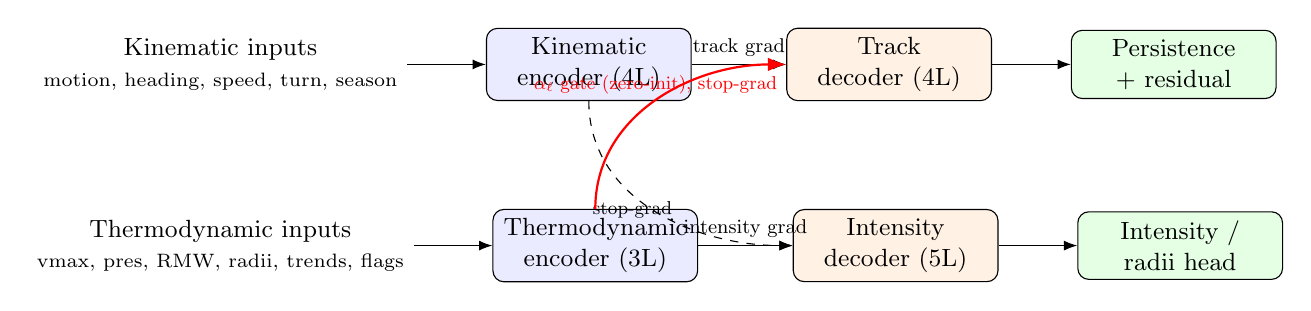
\begin{tikzpicture}[font=\small,>=Latex,node distance=6mm,
  box/.style={draw,rounded corners,minimum height=8mm,minimum width=26mm,align=center},
  enc/.style={box,fill=blue!8}, dec/.style={box,fill=orange!10},
  head/.style={box,fill=green!10}, io/.style={align=center}]
\node[io] (kin) {Kinematic inputs\\{\scriptsize motion, heading, speed, turn, season}};
\node[io,below=14mm of kin] (th) {Thermodynamic inputs\\{\scriptsize vmax, pres, RMW, radii, trends, flags}};
\node[enc,right=10mm of kin] (kenc) {Kinematic\\encoder (4L)};
\node[enc,right=10mm of th] (tenc) {Thermodynamic\\encoder (3L)};
\node[dec,right=12mm of kenc] (tdec) {Track\\decoder (4L)};
\node[dec,right=12mm of tenc] (idec) {Intensity\\decoder (5L)};
\node[head,right=10mm of tdec] (thead) {Persistence\\+ residual};
\node[head,right=10mm of idec] (ihead) {Intensity /\\radii head};
\draw[->] (kin) -- (kenc); \draw[->] (th) -- (tenc);
\draw[->] (kenc) -- node[above,scale=.8]{track grad} (tdec);
\draw[->] (tenc) -- node[above,scale=.8]{intensity grad} (idec);
\draw[->] (tdec) -- (thead); \draw[->] (idec) -- (ihead);
\draw[->,dashed] (kenc.south) to[out=-90,in=180] node[below,scale=.75,pos=.4]{stop-grad} (idec.west);
\draw[->,red,thick] (tenc.north) to[out=90,in=180] node[above,scale=.75,pos=.5]{$\alpha_\ell$ gate (zero-init), stop-grad} (tdec.west);
\end{tikzpicture}
\caption{TrackFormer's protected dual-stream design. Solid arrows carry task gradients back only
into their own encoder; thermodynamics reaches track \emph{only} through a zero-initialized, per-lead
gated adapter on detached features, so at initialization the model is exactly a protected
track-only predictor.}
\label{fig:arch}
\end{figure}

\paragraph{Protected dual-stream architecture.} Kinematic and thermodynamic features are encoded
separately (Figure~\ref{fig:arch}); the track decoder cross-attends only to the kinematic encoding,
and thermodynamics reaches the track head only through a zero-initialized gated adapter,
\begin{equation}
\bm H^{\text{track}}_\ell \;=\; \mathrm{TrackDec}(\bm q_\ell,\bm H^{\text{kin}})
\;+\; \alpha_\ell\,\mathcal A\!\big(\mathrm{sg}(\bar{\bm H}^{\text{th}})\big),
\qquad \alpha_\ell \overset{\text{init}}{=} 0,
\label{eq:gate}
\end{equation}
where $\mathrm{sg}(\cdot)$ is stop-gradient. So intensity can help track (if it lowers track error)
but can never harm it. Track itself is a damped constant-velocity persistence baseline plus a
zero-initialized learned recurvature residual, so the network begins as pure persistence and learns
only the deviation from it. Track loss is a lead-weighted Huber on per-step motion plus a cumulative
Huber, never down-weighted by predicted variance; intensity uses masked Huber $+$ Gaussian NLL with a
monotone wind-radii penalty.

\paragraph{Random-matrix block-structured uncertainty head.} A full $340\times340$ output covariance
is statistically ill-posed and would re-couple track to thermodynamics, so we impose a block-diagonal
$\bm\Sigma=\mathrm{blkdiag}(\bm\Sigma_{\text{track}},\bm\Sigma_{\text{int}},\bm\Sigma_{\text{rad}})$
with a matrix-normal track block and low-rank+diagonal thermodynamic blocks. Sample eigenvalues are
cleaned with a two-point generalized sample-covariance model: the companion Stieltjes transform
solves a cubic
\begin{equation}
a z\,m^3 + \big[a(z-y+1)+z\big]m^2 + \big[a+z-y+1-y\beta(a-1)\big]m + 1 = 0,
\label{eq:cubic}
\end{equation}
whose loss of a real root marks the noise bulk's support edge $\lambda_+$; eigenvalues above
$\lambda_+$ are retained as signal, the rest replaced by a positive floor (setting $a{=}1$ recovers
the classical Marchenko--Pastur edge $\lambda_+=(1+\sqrt y)^2$). Fit on independent storm-block
residuals and applied only after the mean heads converge, this sharpens calibration without touching
the point forecast.

\begin{table}[t]
\centering
\caption{Held-out test performance (lower is better). Track is RMS plane distance over 6--120\,h; the
rest are masked MAE. All models evaluated on identical target windows. Best per column in \textbf{bold}.}
\label{tab:results}
\small
\begin{tabular}{llccccc}
\toprule
split & model & track (km) & vmax (kt) & pres (hPa) & RMW (km) & radius (km)\\
\midrule
WP 2020+
 & single-stream, 40-feat      & \oldWPtrack  & \oldWPvmax  & \oldWPpres  & \oldWPrmw  & \oldWPrad\\
 & single-stream, 48-feat (v2) & \vtwoWPtrack & \vtwoWPvmax & \vtwoWPpres & \vtwoWPrmw & \vtwoWPrad\\
 & TrackFormer (v3)            & \vthreeWPtrack & \vthreeWPvmax & \vthreeWPpres & \vthreeWPrmw & \vthreeWPrad\\
 & TrackFormer (v8, +data)     & \veightWPtrack & \veightWPvmax & \veightWPpres & \veightWPrmw & \veightWPrad\\
 & \textbf{TrackFormer (v9, +env)} & \vnineWPtrack & \vnineWPvmax & \vnineWPpres & \vnineWPrmw & \vnineWPrad\\
\midrule
all-basin 2020+
 & single-stream, 40-feat      & \oldABtrack  & \oldABvmax  & \oldABpres  & \oldABrmw  & \oldABrad\\
 & single-stream, 48-feat (v2) & \vtwoABtrack & \vtwoABvmax & \vtwoABpres & \vtwoABrmw & \vtwoABrad\\
 & TrackFormer (v3)            & \vthreeABtrack & \vthreeABvmax & \vthreeABpres & \vthreeABrmw & \vthreeABrad\\
 & TrackFormer (v8, +data)     & \veightABtrack & \veightABvmax & \veightABpres & \veightABrmw & \veightABrad\\
 & \textbf{TrackFormer (v9, +env)} & \vnineABtrack & \vnineABvmax & \vnineABpres & \vnineABrmw & \vnineABrad\\
\bottomrule
\end{tabular}
\end{table}

\paragraph{Results summary.} The protected architecture (v3) lowers WP-2020+ track from
$\oldWPtrack$ to $659.0$\,km ($-8.5\%$, storm-bootstrap $\Pr(\text{better})=0.995$) while
\emph{improving} intensity/pressure/radius. Keeping partial-lead windows (storm-end/short-storm
fixes, masked rather than discarded) doubled clean training windows and produced v8, best on every
metric ($648.8$\,km WP). Adding a third \emph{environmental} stream of IBTrACS-derived absolute
position, distance-to-land, and a climatological SST proxy --- since the dual-stream model is
translation-invariant and cannot otherwise use latitude (Coriolis, recurvature, SST) --- produced
v9, the best model in this appendix's line ($618.4$\,km WP, $543.4$\,km all-basin; Figure~\ref{fig:storms}).
The consistent lesson: \textbf{data diversity $>$ engineered features $>$ parameters} (a 17.7M
single-stream model overfit and did worse than a 3.3M one; a track-only model matched an ERA5-fed
one). This is what motivated Section~\ref{sec:v10v34}'s environmental-steering branch, this paper's
main subject.

\begin{figure}[t]
\centering
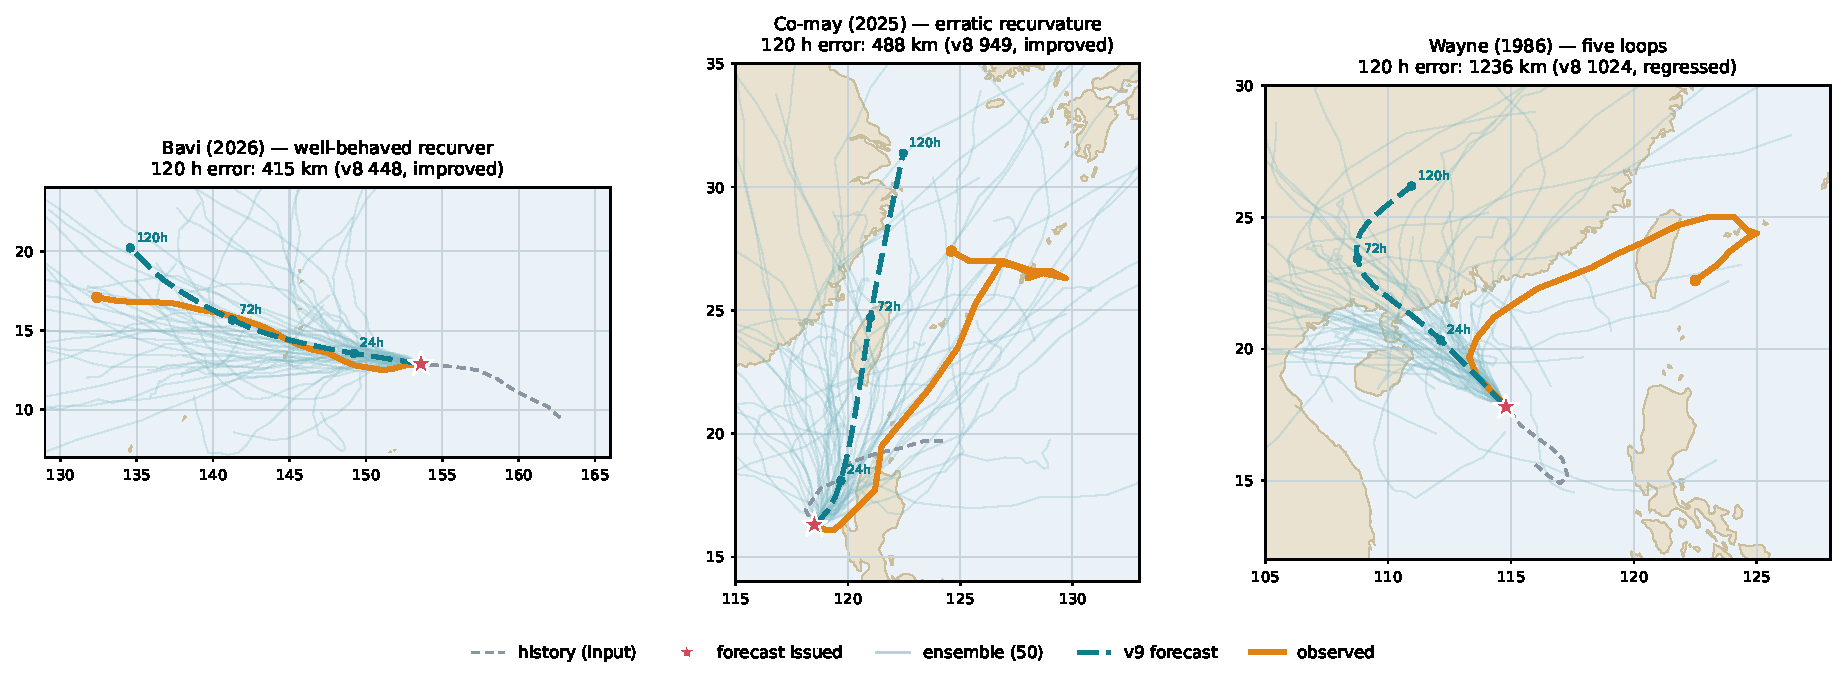
\includegraphics[width=\textwidth]{storms_v9.pdf}
\caption{TrackFormer v9 (triple-stream) on three case studies, each a 120-hour forecast (teal, dashed)
issued from an early fix (star) against the observed track (orange), with the 50-member RMT ensemble
(faint). Absolute latitude sharpens the well-behaved \emph{Bavi} (2026) and \emph{halves} the error on
the erratic \emph{Co-may} (2025), but cannot tame \emph{Wayne}'s (1986) five loops, where climatology
is no substitute for the real-time steering flow. Bavi and Co-may are out-of-sample ($\ge$2020); Wayne
(1986) is in the training window and shown as a stress test.}
\label{fig:storms}
\end{figure}

\end{document}
